\begin{flushleft}
\doublespacing

\subsection{Chancecard - hjælpemetoder}
Da chancekortene(Prøv Lykken kort) arbejder indenfor forskellige kategorier, har vi valgt at opdele dem i IncomeChanceCard, JailChanceCard, MoveChanceCard og PaymentChanceCard klasser. Vi skal have et dæk der kan bruge metoderne fra alle klasserne, så derfor har vi en overordnet klasse der hedder ChanceCard, som alle de nævnte chancekortsklasser nedarver fra. Da de kun nedarver en variabel, har vi valgt at snakke mere om nedarvning i det næste afsnit. I stedet vil vi se på hjælpemetoder der bliver brugt i chancekort klasserne. Da klasserne arbejder indenfor en kategori, har alle metoder i hver klasse en tætlignede funktion. I IncomeChanceCard modtager spilleren et beløb, i MoveChanceCard flytter spilleren position osv. Derfor er der implementeret hjælpemetoder for, at undgå for meget kodereplikation.
Som eksempel vil vi se på IncomeChanceCard. Her har vi lavet to hjælpemetoder. addBalanceFromCard tilføjer penge til spillerens konto, mens receiveMoneyFromOthers giver spilleren et beløb fra hver spiller. De resterende metoder i klasser benytter én af de to hjælpemetoder.
Det kan ses i Figure \ref{IncomeChanceCard assist methods}, at metoderne lotteryCard og stockDividendsCard benytter sig af hjælpemetoden addBalanceFromCard.

\begin{figure}[H] %brug begin{figure} til alle figurer.
    \centering
    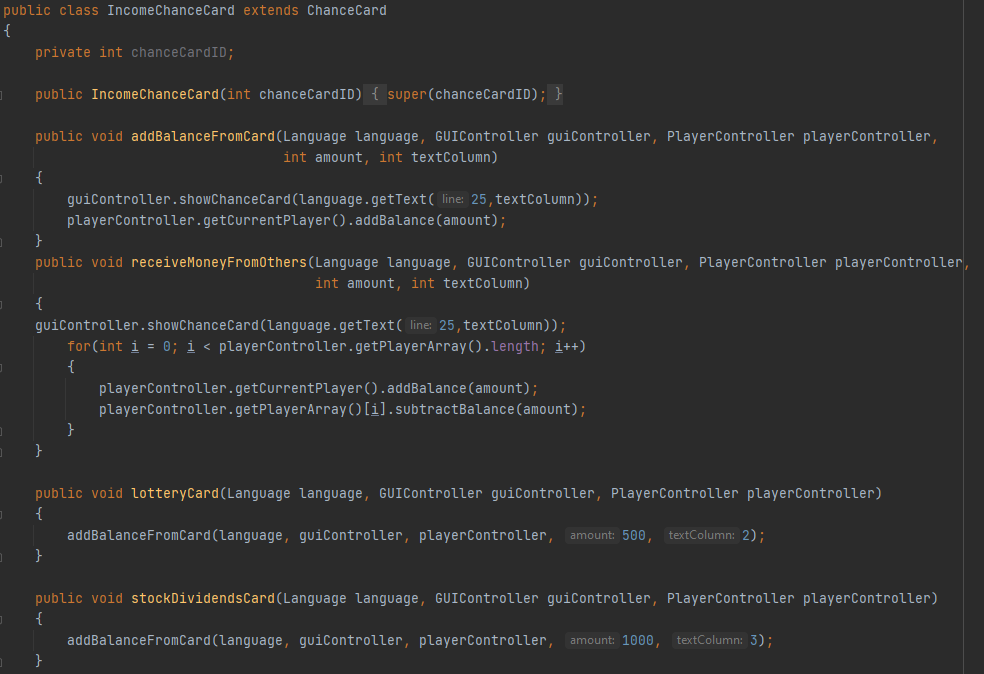
\includegraphics[width=14cm]{Report/figures/Codesections/IncomeChanceCard_addBalanceFromCard()+receiveMoneyFromOthers().PNG}
    \caption{Hjælpemetoder i IncomeChanceCard}
    \label{IncomeChanceCard assist methods}
\end{figure}


\subsection{Fields - nedarvning og polymorphism}
I Field klassen (se Figure \ref{Field_constructor}) har vi gjort klassen abstract, så der ikke kan dannes objekter af klassen, men kun af nedarvede klasser for Field. Vi bruger protected som access modifier for instansvariablerne, så de kan tilgås af nedarvede klasser.
\begin{figure}[H] %brug begin{figure} til alle figurer.
    \centering
    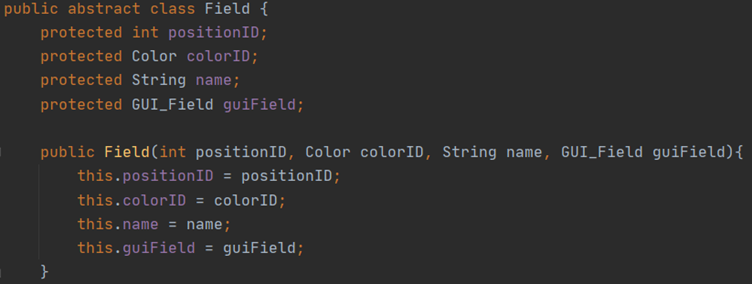
\includegraphics[width=14cm]{Report/figures/Codesections/Field_constructor().png}
    \caption{Field klassens konstruktør}
    \label{Field_constructor}
\end{figure}

I BuyableField klassen det ses, at klassen nedarver fra Field klassen (se Figure \ref{BuyableField_constructor}). Her bruges super() variable til at referere til objekt instanser fra dens parent class, Field. Det ses yderligere, at vi igen bruger abstract klassen - dette er fordi BuyableField er yderligere nedarvet af flere klasser, hvor vi ikke ønsker, at der kan laves objekter direkte af BuyableField.
    
\begin{figure}[H]
    \centering
    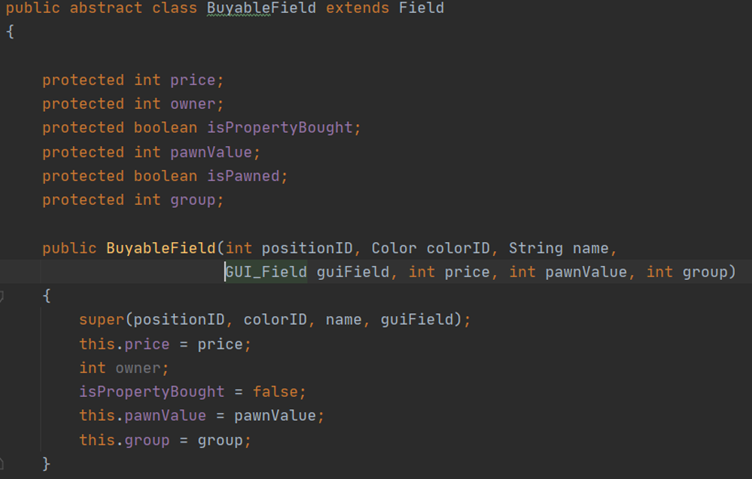
\includegraphics[width=14cm]{Report/figures/Codesections/BuyableField_constructor().png}
    \caption{BuyableField klassens konstruktør}
    \label{BuyableField_constructor}
\end{figure}

I Field klassen ses det yderligere, at der findes an abstract metode, landOnField() (se Figure \ref{Field_landOnField}). Dette vil sige, at metoden skal defineres i de nedarvede klasser af Field og ikke indeholder en body, da denne specificeres af de nedarvede klasser.

\begin{figure}[H]
    \centering
    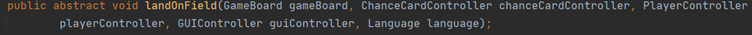
\includegraphics[width=14cm]{Report/figures/Codesections/Field_landOnField().png}
    \caption{Field klassens landOnField() metode}
    \label{Field_landOnField}
\end{figure}

I JailField klassen kan man se et eksempel på polymorphism af metoden landOnField(), som er nedarvet fra Field klassen. Herved bliver logikken i landOnField() anderledes i JailField klassen fra sine sibling-classes. 
    
\begin{figure}[H]
    \centering
    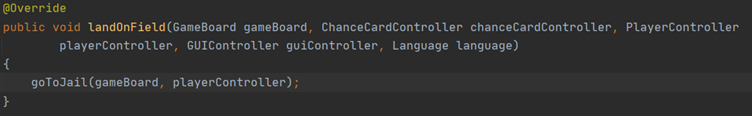
\includegraphics[width=14cm]{Report/figures/Codesections/BuyAbleField_landOnField().png}
    \caption{JailField klassens landOnField() metode}
    \label{Jailfield_landOnField}
\end{figure}

\subsection{Language - 2D array, tekstfil og try/catch}
Language klassen bruges til at indlæse Strings fra en csv fil et 2D array, hvor linjetallet i csv filen bliver indlæst i første dimension af String[][] ImportedText mens String objekterne bliver indlæst i anden dimension af ImportedText. Herved sikrer vi os, at det er nemt at ændre i tekstfilen og lave andre versioner af den - f.eks. hvis man ønsker at oversætte hele tekstfilen til et andet sprog. Yderligere bruger vi try/catch statements til at udskrive en error, hvis filen ikke bliver fundet. For at hente teksten, der bliver indlæst fra filen, kan man bruge metoden getText, hvor der indsættes to heltal som parametre, der svarer til hhv. linjen og kolonnen i csv filen.
\begin{figure}[htp] %brug begin{figure} til alle figurer.
    \centering
    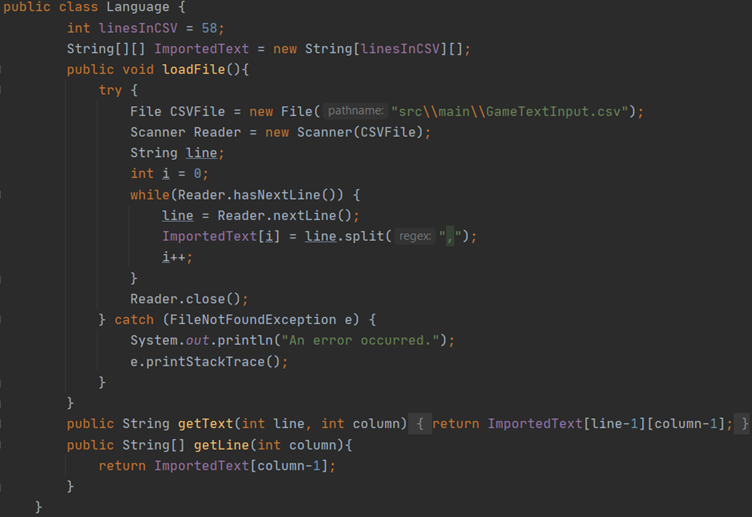
\includegraphics[width=14cm]{Report/figures/Codesections/Language_Language.png}
    \caption{Oversigt af Language klassen}
    \label{LanguageKlasse}
\end{figure}

\subsection{Menu - instanceOf og expandable array}
I klassen Menu, er der lavet metoderne expandArr og expandStrArr. Disse to metoder udvider et modtaget array med én. Dermed har vi mulighed for at udvide arrays. Når der skal ses hvilke grunde der kan købes huse elller hotel på, og hvilke man ejer og kan pantsætte osv. kan man gå alle felterne igennem, og hver gang man finder en felt der matcher ens beskrivelse, da tilføje dem til et array der bliver én større for hver gang (se Figure \ref{Expanding arrays}).

\begin{figure}[H] %brug begin{figure} til alle figurer.
    \centering
    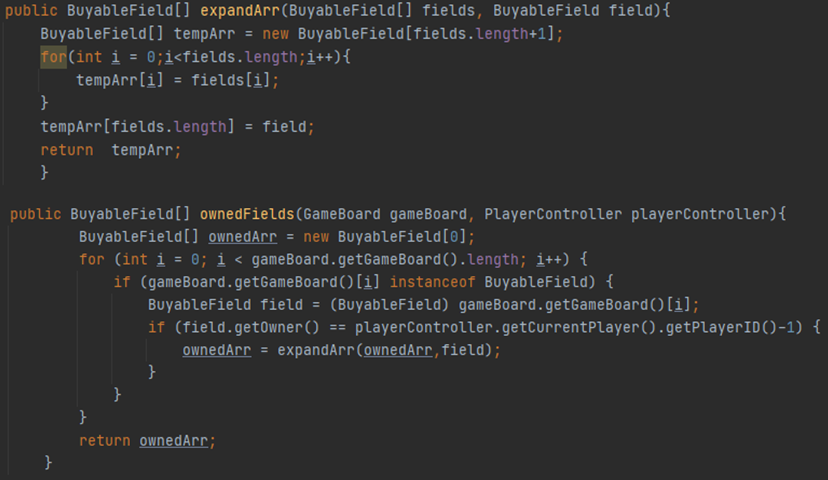
\includegraphics[width=14cm]{Report/figures/Codesections/Menu_expandArr()+ownedFields().PNG}
    \caption{Metoderne expandArr og ownedFields der benytter expandArr}
    \label{Expanding arrays}
\end{figure}


\end{flushleft}